\documentclass[usenames,dvipsnames,8pt]{beamer}
\usepackage{booktabs}

\usepackage{sagetex}
\usepackage{header100}
\usepackage{nicefrac}

\usetikzlibrary{patterns}
%\pgfplotsset{compat=1.15}
\pgfplotsset{compat=newest}
\pgfplotsset{
  integral segments/.code={\pgfmathsetmacro\integralsegments{#1}},
  integral segments=3,
  integral samples/.code={\edef\integralsamples{#1}},
  integral samples = 10,
  integral min/.style args={#1:#2}{
    ybar interval,
    domain=#1:#2,
    samples=\integralsegments+1,
    x filter/.code={
      \edef\lastx{\pgfmathresult}
      \pgfmathresult
    },%
    y filter/.code={%
      \pgfmathparse{(#2/(\integralsegments))/\integralsamples}%
      \edef\tempstep{\pgfmathresult}%
      \pgfmathparse{f(\lastx)}%
      \edef\tempa{\pgfmathresult}%
      \edef\tempb{\pgfmathresult}%
      \foreach \x in {0,1,...,\integralsamples}%
        {%
          \pgfmathparse{f(\lastx+\x*\tempstep)}%
          \xdef\tempb{\tempb,\pgfmathresult}%
        }%
        \pgfmathmin{\tempb}{\tempb}
        \let\savepgfmathresult\pgfmathresult
        \pgfmathgreater{\pgfmathresult}{0}
        \ifdim\pgfmathresult pt> 0 pt \relax
        \let\pgfmathresult\savepgfmathresult 
        \else
        \pgfmathparse{f(\lastx)}%
        \edef\tempa{\pgfmathresult}%
        \edef\tempb{\pgfmathresult}%
        \foreach \x in {0,1,...,\integralsamples}%
          {%
            \pgfmathparse{f(\lastx+\x*\tempstep)}%
            \xdef\tempb{\tempb,\pgfmathresult}%
          }%
          \pgfmathmax{\tempb}{\tempb}
        \fi 
      },
    },
    integral max/.style args={#1:#2}{
      ybar interval,
      domain=#1:#2,
      samples=\integralsegments+1,
      x filter/.code={
        \edef\lastx{\pgfmathresult}
        \pgfmathresult
      },%
      y filter/.code={%
        \pgfmathparse{(#2/(\integralsegments))/\integralsamples}%
        \edef\tempstep{\pgfmathresult}%
        \pgfmathparse{f(\lastx)}%
        \edef\tempa{\pgfmathresult}%
        \edef\tempb{\pgfmathresult}%
        \foreach \x in {0,1,...,\integralsamples}%
        {%
          \pgfmathparse{f(\lastx+\x*\tempstep)}%
          \xdef\tempb{\tempb,\pgfmathresult}%
        }%
        \pgfmathmax{\tempb}{\tempb,0}
        \let\savepgfmathresult\pgfmathresult
%       \pgfmathparse{ifthenelse(\pgfmathresult>=0,1,0)} 
        \pgfmathgreater{\pgfmathresult}{0}
        \ifdim\pgfmathresult pt> 0 pt \relax
        \let\pgfmathresult\savepgfmathresult 
        \else
        \pgfmathparse{f(\lastx)}%
        \edef\tempa{\pgfmathresult}%
        \edef\tempb{\pgfmathresult}%
        \foreach \x in {0,1,...,\integralsamples}%
          {%
            \pgfmathparse{f(\lastx+\x*\tempstep)}%
            \xdef\tempb{\tempb,\pgfmathresult}%
          }%
        \pgfmathmin{\tempb}{\tempb}
      \fi 
    },
  },   
}
\makeatletter
%see https://tex.stackexchange.com/questions/9722/why-am-i-getting-the-pgf-math-error-unknown-function-getargs
\def\pgfmathmax#1#2{%
%   \pgfmathparse{getargs(#1,#2)}%
     \pgfmathparse{#1,#2}%
    \expandafter\pgfmathmax@\expandafter{\pgfmathresult}%
}
\def\pgfmathmin#1#2{%
    \pgfmathparse{#1,#2}%
    \expandafter\pgfmathmin@\expandafter{\pgfmathresult}%
}
%see https://tex.stackexchange.com/questions/15435/how-do-i-use-pgfmathdeclarefunction-to-create-define-a-new-pgf-function
\makeatother

%\usepackage{clp_notes_header}
%\graphicspath{{./figures/misc/}}

\usepackage{unicode-math}
\usepackage[BoldFont,SlantFont]{xeCJK}  
\xeCJKsetemboldenfactor{2}
%\setCJKmainfont{cwTeX Q Kai Medium}
%\setCJKmainfont{cwTeX Q Ming Medium}
\setCJKmainfont{cwTeX Q Yuan Medium}
%\usepackage[AutoFakeBold,AutoFakeSlant]{xeCJK}  
%\setCJKmainfont[AutoFakeSlant=.1,AutoFakeBold=1]{cwTeX Q Kai Medium} 
%\setCJKfamilyfont{kaiv}[Vertical=RotatedGlyphs]{cwTeX Q Medium}
\setmainfont{texgyrepagella-regular.otf}
\setmathfont{texgyrepagella-math.otf}
\usepackage{datetime2}

\usepackage{enumitem}

\usetheme{Madrid}
\usecolortheme{beaver}

% XXX https://tex.stackexchange.com/questions/216435/how-do-i-properly-label-the-figures-and-tables-in-beamer-in-share-latex
\setbeamertemplate{caption}[numbered]{} % Number float-like environments

\setbeamertemplate{footline}[text line]{%
  \parbox{\linewidth}{\vspace*{-8pt}
  \DTMnow\hfill\href{https://github.com/chang-ye-tu/calc}{https://github.com/chang-ye-tu/calc}\hfill
  \hyperlink{toc}{TOC} ~~ \insertframenumber / \inserttotalframenumber~~~~~~~~~}}
\setbeamertemplate{navigation symbols}[only frame symbol]

% white letters in enumerate bullet points
%\definecolor{stupidblue}{RGB}{51,51,178}
\setbeamercolor{item projected}{fg=white}%fg=blue,bg=red!75!black} % fg=white , bg=stupidblue
\setbeamercolor{frametitle}{fg=black}
% Block title color
\setbeamercolor{block title}{fg=white}%fg=blue,bg=red!75!black} % white
%\setbeamertemplate{item projected}[square]

\definecolor{foo}{rgb}{.2,.2,.7}
\AtBeginSection[]{
  \begin{frame}
  \vfill
  \centering
  \begin{beamercolorbox}[sep=8pt,center,shadow=true,rounded=true]{section page}
    \usebeamerfont{title}%
    {\color{foo} \insertsectionhead}\par%
  \end{beamercolorbox}
  \vfill
  \end{frame}
}

% https://tex.stackexchange.com/questions/30423/bibliography-in-beamer
\setbeamertemplate{bibliography entry title}{}
\setbeamertemplate{bibliography entry location}{}
\setbeamertemplate{bibliography entry note}{}

\DeclareMathOperator\prb{{\sf P}}
\DeclareMathOperator\expc{{\sf E}}
\DeclareMathOperator\var{var}
\DeclareMathOperator\cov{cov}
\DeclareMathOperator*{\argmax}{\arg\!\max}
\DeclareMathOperator*{\argmin}{\arg\!\min}
\DeclareMathOperator\corr{corr}
\DeclareMathOperator\rk{rank}
\DeclareMathOperator\sgn{sgn}

\usepackage{dsfont} % indicator function \mathds{1}
\DeclareMathOperator\indc{\mathds{1}}

\newbool{render}
%\booltrue{render}
\newbool{integral}

\setbeamertemplate{headline}{}
\title{Calculus}
%\author{Chang-Ye Tu}
\author{}
\date{}%\today}

\begin{document}

\begin{frame}
  \titlepage
\end{frame}

\subsection*{Outline}
\begin{frame}
  \tableofcontents
\end{frame}

%\ifbool{render}{

\section{L'H\^opital's Rule}

\begin{frame}
  \frametitle{Intermediate Forms}
  \begin{table}[!htbp]
    \centering
    \caption{\onslide<+->{Typical Intermediate Forms of Limit}}
    \begin{tabular}{cc} \toprule
      Form & Example \\
      \midrule
      \onslide<+->{$\displaystyle\frac{0}{0}$} & \onslide<+->{$\displaystyle\lim_{x\to 0}\frac{\sin x}{x}$ \\}  
      \onslide<+->{$\displaystyle\frac{\infty}{\infty}$} & \onslide<+->{$\displaystyle\lim_{x\to 0}\frac{\ln\frac{1}{x^2}}{\cot x^2}$ \\}  
      \onslide<+->{$\displaystyle 0\cdot\infty$} & \onslide<+->{$\displaystyle\lim_{x\to 0+}x\ln\frac{1}{x}$ \\}  
      \onslide<+->{$\displaystyle \infty - \infty$} & \onslide<+->{$\displaystyle\lim_{x\to\frac{\pi}{2}-}\Big(\tan x - \frac{1}{\pi - 2x}\Big)$ \\}  
      \onslide<+->{$\displaystyle 0^0$} & \onslide<+->{$\displaystyle\lim_{x\to 0+} x^x$ \\}  
      \onslide<+->{$\displaystyle \infty^0$} & \onslide<+->{$\displaystyle\lim_{x\to \frac{\pi}{2}-} (\tan x)^{\cos x}$ \\}  
      \onslide<+->{$\displaystyle 1^\infty$} & \onslide<+->{$\displaystyle\lim_{x\to\infty} \Big(1 + \frac{1}{x}\Big)^x$ \\ \bottomrule}  
    \end{tabular}
  \end{table}
  \begin{itemize}
    \item We will focus on $\displaystyle\frac{0}{0}, \frac{\infty}{\infty}$; Other forms can sometimes be transformed to these two
  \end{itemize}
\end{frame}

\begin{frame}
  \frametitle{L'H\^opital's Rule: Statement}
  \begin{itemize}
    \item Let $f$ and $g$ be real-valued and differentiable with
      \begin{align}\label{ne}\tag{Denominator' $\ne 0$}
        \onslide<+->{g'\ne 0}
      \end{align}
      on $(a, b)$, $a < b$, $a, b\in\mathbb{R}^\sharp$. Suppose
      \begin{align}\label{zero2}\tag{$\displaystyle\frac{0}{0}$}
        \onslide<+->{\lim_{x\downarrow a} f(x) = \lim_{x\downarrow a} g(x) = 0} 
      \end{align}
      or
      \begin{align}\label{inftyg}\tag{Denominator $=\infty$}
        \onslide<+->{\lim_{x\downarrow a} g(x) = \infty} 
      \end{align}
      \onslide<+->{If
        \begin{align*}
          \lim_{x\downarrow a} \frac{f'(x)}{g'(x)} = L\in\mathbb{R}^\sharp
        \end{align*}}
      \onslide<+->{Then
        \begin{align*}
          \lim_{x\downarrow a} \frac{f(x)}{g(x)} = L
        \end{align*}}
      \onslide<+->{The result holds if $x\downarrow a$ is replaced by $x\uparrow b$ and/or $\infty$ is replaced by $-\infty$.}
  \end{itemize}
\end{frame}

\begin{frame}
  \frametitle{L'H\^opital's Rule: Example I}
  \begin{itemize}
    \item Find
      \begin{align*}
        \onslide<+->{\lim_{x\to 0}\frac{\sin x}{x}}
      \end{align*}
    \onslide<+->{\item We know from trigonometric considerations $\displaystyle \lim_{x\to 0}\frac{\sin x}{x} = 1$}
    \onslide<+->{\item Now using L'H\^opital's rule by checking the conditions \eqref{ne} and \eqref{zero2}:}
    \onslide<+->{\item \eqref{ne} $(x)' = 1\ne 0$ on $(0, b)$, $b > 0$.}
    \onslide<+->{\item \eqref{zero2} $\displaystyle\lim_{x\to 0}\frac{\sin x}{x}$ is of $\displaystyle\frac{0}{0}$ form: $\displaystyle\lim_{x\to 0}\sin x = \lim_{x\to0} x = 0$}
    \onslide<+->{\item Hence $$\lim_{x\to 0}\frac{\sin x}{x} = \lim_{x\to 0}\frac{(\sin x)'}{(x)'} = \lim_{x\to 0}\frac{\cos x}{1} = 1$$}
  \end{itemize}
\end{frame}

\begin{frame}
  \frametitle{L'H\^opital's Rule: Example II}
  \begin{itemize}
    \item Find
      \begin{align*}
        \onslide<+->{\lim_{x\to\infty}\,\frac{\ln x}{x^\alpha}, \quad\alpha > 0}
      \end{align*}
      \onslide<+->{\item We know from previous class $\displaystyle \lim_{x\to\infty}\frac{\ln x}{x^\alpha} = 0$ by using $\ln x\leqslant x - 1$, $\forall x>0$.}
    \onslide<+->{\item Now using L'H\^opital's rule by checking the conditions \eqref{ne} and \eqref{inftyg}:}
    \onslide<+->{\item \eqref{ne} $(x^\alpha)' = \alpha x^{\alpha - 1}\ne 0$ on $(a, \infty)$, $a > 0$.}
    \onslide<+->{\item \eqref{inftyg} $\displaystyle\lim_{x\to\infty} x^\alpha = \infty$}
    \onslide<+->{\item Hence $$\lim_{x\to\infty}\frac{\ln x}{x^\alpha} = \lim_{x\to\infty}\frac{(\ln x)'}{(x^\alpha)'} = \lim_{x\to\infty}\frac{\frac{1}{x}}{\alpha x^{\alpha-1}} = \lim_{x\to\infty}\frac{1}{\alpha x^\alpha} = 0$$}
  \end{itemize}
\end{frame}

\begin{frame}
  \frametitle{L'H\^opital's Rule: Example III}
  \begin{itemize}
    \item Find
      \begin{align*}
        \onslide<+->{\lim_{x\to1+}\bigg(\frac{x}{x - 1} - \frac{1}{\ln x}\bigg)}
      \end{align*}
    \onslide<+->{\item This is of the form $\infty - \infty$; Need to be transformed before using L'H\^opital's rule}
    \onslide<+->{\item $$\lim_{x\to1+}\bigg(\frac{x}{x - 1} - \frac{1}{\ln x}\bigg) = \lim_{x\to1+}\frac{x\ln x - (x - 1)}{(x - 1)\ln x}\qquad\text{(In the form $\frac{0}{0}$)}$$}
    \onslide<+->{\item Now using L'H\^opital's rule by checking the conditions \eqref{ne} and \eqref{zero2}:}
    \onslide<+->{\item \eqref{ne} $\displaystyle((x-1)\ln x)' = 1 - \frac{1}{x} + \ln x\ne 0$ on $(1, b)$, $b > 1$.}
    \onslide<+->{\item \eqref{zero2} $\displaystyle\lim_{x\to1+}\frac{x\ln x - (x - 1)}{(x - 1)\ln x}$ is of $\displaystyle\frac{0}{0}$ form: $\displaystyle\lim_{x\to1+}x\ln x - (x - 1) = \lim_{x\to1+}(x - 1)\ln x = 0$}
    \onslide<+->{\item Hence} 
      \begin{align*}
        \onslide<+->{\lim_{x\to1+}\frac{x\ln x - (x - 1)}{(x - 1)\ln x} = \lim_{x\to1+}\frac{(x\ln x - (x - 1))'}{((x - 1)\ln x)'}}\onslide<+->{= \lim_{x\to1+}\frac{1 + \ln x - 1}{1-\frac{1}{x} + \ln x} = \lim_{x\to1+}\frac{\ln x}{1 - \frac{1}{x} + \ln x}}
      \end{align*}
  \end{itemize}
\end{frame}

\begin{frame}
  \frametitle{L'H\^opital's Rule: Example III (Cont'd)}
  \begin{itemize}
    \item Using L'H\^opital's rule again with
      \begin{align*}
        \onslide<+->{\lim_{x\to1+}\frac{\ln x}{1 - \frac{1}{x} + \ln x}}
      \end{align*}
    \onslide<+->{\item Checking the conditions \eqref{ne} and \eqref{zero2}:}
    \onslide<+->{\item \eqref{ne} $\displaystyle\Big(1 - \frac{1}{x} + \ln x\Big)' = \frac{1 + x}{x^2} \ne 0$ on $(1, b)$, $b > 1$.}
    \onslide<+->{\item \eqref{zero2} $\displaystyle\lim_{x\to1+}\frac{\ln x}{1 - \frac{1}{x} + \ln x}$ is of $\displaystyle\frac{0}{0}$ form: $\displaystyle\lim_{x\to1+}\ln x= \lim_{x\to1+}1 - \frac{1}{x} + \ln x = 0$}
    \onslide<+->{\item Hence} 
      \begin{align*}
        \onslide<+->{\lim_{x\to1+}\frac{\ln x}{1 - \frac{1}{x} + \ln x} = \lim_{x\to1+}\frac{(\ln x)'}{\Big(1 - \frac{1}{x} + \ln x\Big)'}}\onslide<+->{= \lim_{x\to1+}\frac{\frac{1}{x}}{\frac{1 + x}{x^2}} = \frac{1}{2}}
      \end{align*}
    \onslide<+->{\item So
      \begin{align*}
        \lim_{x\to1+}\bigg(\frac{x}{x - 1} - \frac{1}{\ln x}\bigg) = \lim_{x\to1+}\frac{x\ln x - (x - 1)}{(x - 1)\ln x} = \lim_{x\to1+}\frac{\ln x}{1 - \frac{1}{x} + \ln x} = \frac{1}{2}
    \end{align*}}
  \end{itemize}
\end{frame}

\begin{frame}
  \frametitle{L'H\^opital's Rule: Example IV}
  \begin{itemize}
    \item Find 
      \begin{align*}
        \onslide<+->{\lim_{x\to0}\,\bigg(\frac{\sin x}{x}\bigg)^{\frac{1}{x^2}}}
      \end{align*}
    \onslide<+->{\item This is of the form $1^\infty$; Need to be transformed before using L'H\^opital's rule}
    \onslide<+->{\item We consider the logarithm $$\lim_{x\to0}\frac{1}{x^2}\ln\frac{\sin x}{x} = \lim_{x\to0}\frac{\ln\frac{\sin x}{x}}{x^2}\qquad\text{(In the form $\frac{0}{0}$)}$$ and get back to the orginal limit by exponentiation}
    \onslide<+->{\item Now using L'H\^opital's rule by checking the conditions \eqref{ne} and \eqref{zero2}:}
    \onslide<+->{\item \eqref{ne} $\displaystyle(x^2)' = 2x\ne 0$ on $(0, b)$, $b > 0$.}
    \onslide<+->{\item \eqref{zero2} $\displaystyle\lim_{x\to0}\frac{\ln\frac{\sin x}{x}}{x^2}$ is of $\displaystyle\frac{0}{0}$ form: $\displaystyle\lim_{x\to0}\ln\frac{\sin x}{x} = \lim_{x\to0}x^2 = 0$}
    \onslide<+->{\item Hence} 
      \begin{align*}
      \onslide<+->{\lim_{x\to0}\frac{\ln\frac{\sin x}{x}}{x^2} = \lim_{x\to0}\frac{\Big(\ln\frac{\sin x}{x}\Big)'}{(x^2)'}}\onslide<+->{= \lim_{x\to0}\frac{\frac{x}{\sin x}\frac{(x\cos x - \sin x)}{x^2}}{2x} = \lim_{x\to0}\frac{x\cos x - \sin x}{2 x^2\sin x}}
      \end{align*}
  \end{itemize}
\end{frame}

\begin{frame}
  \frametitle{L'H\^opital's Rule: Example IV (Cont'd)}
  \begin{itemize}
    \item Using L'H\^opital's rule again with
      \begin{align*}
        \onslide<+->{\lim_{x\to0}\frac{x\cos x - \sin x}{2 x^2\sin x}}
      \end{align*}
    \onslide<+->{\item Checking the conditions \eqref{ne} and \eqref{zero2}:}
    \onslide<+->{\item \eqref{ne} $\displaystyle(2 x^2\sin x)' = 2x^2\cos x + 4x\sin x\ne 0$ on $(0, b)$, $b > 0$ is small.}
    \onslide<+->{\item \eqref{zero2} $\displaystyle\lim_{x\to0}\frac{x\cos x - \sin x}{2 x^2\sin x}$ is of $\displaystyle\frac{0}{0}$ form: $\displaystyle\lim_{x\to0}(x\cos x - \sin x) = \lim_{x\to0}2x^2\sin x = 0$}
    \onslide<+->{\item Hence} 
      \begin{align*}
        \onslide<+->{\lim_{x\to0}\frac{x\cos x - \sin x}{2 x^2\sin x} = \lim_{x\to0}\frac{(x\cos x - \sin x)'}{(2 x^2\sin x)'}}\onslide<+->{= \lim_{x\to0}\frac{- x\sin x}{2x^2\cos x + 4x\sin x} = \lim_{x\to0}\frac{-\sin x}{2 x\cos x + 4\sin x}}
      \end{align*}
  \end{itemize}
\end{frame}

\begin{frame}
  \frametitle{L'H\^opital's Rule: Example IV (Cont'd)}
  \begin{itemize}
    \item Using L'H\^opital's rule again with
      \begin{align*}
        \onslide<+->{\lim_{x\to0}\frac{-\sin x}{2 x\cos x + 4\sin x}}
      \end{align*}
    \onslide<+->{\item Checking the conditions \eqref{ne} and \eqref{zero2}:}
    \onslide<+->{\item \eqref{ne} $\displaystyle(2 x\cos x + 4\sin x)' = -2x\sin x + 6\cos x\ne 0$ on $(0, b)$, $b > 0$ is small.}
    \onslide<+->{\item \eqref{zero2} $\displaystyle\lim_{x\to0}\frac{-\sin x}{2 x\cos x + 4\sin x}$ is of $\displaystyle\frac{0}{0}$ form: $\displaystyle\lim_{x\to0}(-\sin x) = \lim_{x\to0}(2x\cos x + 4\sin x) = 0$}
    \onslide<+->{\item Hence} 
      \begin{align*}
        \onslide<+->{\lim_{x\to0}\frac{-\sin x}{2 x\cos x + 4\sin x} = \lim_{x\to0}\frac{(-\sin x)'}{(2 x\cos x + 4\sin x)'}}\onslide<+->{= \lim_{x\to0}\frac{-\cos x}{-2x\sin x + 6\cos x} = -\frac{1}{6}}
      \end{align*}
    \onslide<+->{\item So
      \begin{multline*}
        \lim_{x\to0}\,\bigg(\frac{\sin x}{x}\bigg)^{\frac{1}{x^2}} = \exp\Bigg\{\lim_{x\to0}\frac{1}{x^2}\ln\frac{\sin x}{x}\Bigg\} \\= \exp\Bigg\{\lim_{x\to0}\frac{x\cos x - \sin x}{2 x^2\sin x}\Bigg\} = \exp\Bigg\{\lim_{x\to0}\frac{-\sin x}{2 x\cos x + 4\sin x}\Bigg\} = e^{-\frac{1}{6}}
    \end{multline*}}
  \end{itemize}
\end{frame}

\begin{frame}
  \frametitle{L'H\^opital's Rule: Exercises}
  \begin{itemize}
    \item (4.3.29)
      \begin{align*}
        \lim_{x\to 0}\,(\cos 2x)^{\frac{1}{x^2}}
      \end{align*}
    \item (4.3.30)
      \begin{align*}
        \lim_{x\to 0+}\frac{\csc x}{\ln x}
      \end{align*}
    \item (4.3.31)
      \begin{align*}
        \lim_{x\to 0}\frac{\ln\sin\pi x}{\csc\pi x}
      \end{align*}
    \item (4.3.32)
      \begin{align*}
        \lim_{x\to 0}\,(1 + \tan x)^{\frac{1}{x}}
      \end{align*}
    \item (4.3.33) For twice differentiable $f$, find 
      \begin{align*}
        \lim_{h\to 0}\frac{f(x + h) - 2 f(x) + f(x - h)}{h^2}
      \end{align*}
    \item (4.3.34) If $f$ has continuous third derivative, find
      \begin{align*}
        \lim_{h\to 0}\frac{f(x + 3h) - 3 f(x + h) + 3f(x - h) - f(x - 3h)}{h^3}
      \end{align*}
  \end{itemize}
\end{frame}

%\begin{frame}
%  \frametitle{L'H\^opital's Rule: Proof}
%\end{frame}

\section{Extreme Values}

\begin{frame}
  \frametitle{Maximum and Minimum Values}
  \begin{itemize}
    \item \onslide<+->{Let $f:I\mapsto\mathbb{R}$.} 
      \begin{itemize}
        \vfill\item \onslide<+->{$f$ has an absolute maximum value $f(x_0)$ at $x_0\in I$ if }\onslide<+->{ $f(x) \leqslant f(x_0)\quad\forall x\in I$}
        \vfill\item \onslide<+->{$f$ has an absolute minimum value $f(x_1)$ at $x_1\in I$ if }\onslide<+->{ $f(x) \geqslant f(x_1)\quad\forall x\in I$}
        \vfill\item \onslide<+->{$f$ has an local maximum value $f(x_0)$ at $x_0\in I$ if }\onslide<+->{ $\exists\,h > 0$ s.t. $f(x) \leqslant f(x_0)\quad\forall x\in I$, $|x - x_0| < h$.}
        \vfill\item \onslide<+->{$f$ has an local minimum value $f(x_1)$ at $x_1\in I$ if }\onslide<+->{ $\exists\,h > 0$ s.t. $f(x) \geqslant f(x_1)\quad\forall x\in I$, $|x - x_1| < h$.}
      \end{itemize}

    \vfill\item \onslide<+->{Examples:}
      \begin{itemize}
        \vfill\item \onslide<+->{$f(x) = \sin x$ on $I=\mathbb{R}$}\onslide<+->{ has absolute maximum $1$ and absolute minimum $-1$} 
        \vfill\item \onslide<+->{$f(x) = \frac{1}{x}$ on $I=\mathbb{R}$}\onslide<+->{ has no absolute maximum and minimum} 
        \vfill\item \onslide<+->{$f(x) = x$ on $I=(0, 1)$}\onslide<+->{ has no absolute maximum and minimum} 
        \vfill\item \onslide<+->{$f(x) = x$ on $I=[0, 1]$}\onslide<+->{ has absolute maximum $1$ and minimum $0$} 
      \end{itemize}

    \vfill\item\onslide<+->{Theorem: If $f$ is defined and continuous on }
      \begin{itemize}
        \vfill\item \onslide<+->{1. a closed, finite interval}
        \vfill\item \onslide<+->{2. a union of finitely many such interval} 
      \end{itemize}
      \onslide<+->{then $f$ has absolute maximum and minimum.}
  \end{itemize}
\end{frame}

\begin{frame}
  \frametitle{Critical Points, Singular Points, and Endpoints}
  \begin{itemize}
    \item \onslide<+->{Theorem: Let $f:I\mapsto\mathbb{R}$ and has a local extremum (maximum or minimum) value at $x=x_0\in I$, then $x_0$ must be either }
      \begin{itemize}
        \vfill\item \onslide<+->{1. a critical point (zero derivatives) }
        \vfill\item \onslide<+->{2. a singular point (discontinuous / nondifferentiable) }
        \vfill\item \onslide<+->{3. an endpoint of $I$}
      \end{itemize}

    \vfill\item \onslide<+->{Example: Find the maximum and minimum values of the function $f(x) = x^3 - 3 x^2 - 9 x + 2$ on $[-2, 2]$.}
      \begin{itemize}
        \vfill\item \onslide<+->{$f(x)$ has no singular points, for $f(x)$ is a polynomial.}
        \vfill\item \onslide<+->{$f'(x) = 3 x^2 - 6 x - 9 = 3(x + 1)(x - 3)$, so $f'(-1) = 0$.}
        \vfill\item \onslide<+->{The extremum is obtained among the endpoints $x = -2, 2$ and the critical point $x = -1$.}
        \vfill\item \onslide<+->{The maximum is $f(-1) = 7$, the minimum is $f(2) = -20$.}
      \end{itemize}
  \end{itemize}
\end{frame}

\begin{frame}
  \frametitle{Functions Not Defined on Closed, Finite Intervals}
  \begin{itemize}
    \item\onslide<+->{Theorem: If $f$ is continuous on $(a, b)$ and $\lim_{x\to a+}f(x) = L$, $\lim_{x\to b-}f(x) = M$. Then}
      \begin{itemize}
        \vfill\item \onslide<+->{If $f(u) > L$ and $f(u) > M$ for some $u\in(a, b)$, then $f$ has an absolute maximum value on $(a, b)$.}
        \vfill\item \onslide<+->{If $f(v) < L$ and $f(v) < M$ for some $v\in(a, b)$, then $f$ has an absolute minimum value on $(a, b)$.}
        \vfill\item \onslide<+->{\hypertarget{thm:opt}{$a$ may be $-\infty$, $b$ may be $\infty$, $L$, $M$ may be $-\infty$, $\infty$.}}
      \end{itemize}

    \vfill\item \onslide<+->{Example: Show that $f(x) = x + \frac{4}{x}$ on $(0, \infty)$ has an absolute minimum value, and find it.}
      \begin{itemize}
        \vfill\item \onslide<+->{$\lim_{x\to 0+}f(x) = \infty$, $\lim_{x\to\infty}f(x) = \infty$, and $f(1) = 5$.}
        \vfill\item \onslide<+->{From theorem above, $f$ has an absolute minimum value on $(0, \infty)$.}
        \vfill\item \onslide<+->{The extremum is obtained among the critical points.}
        \vfill\item \onslide<+->{$f'(x) = 1 + 4 (-x^{-2}) = \frac{(x + 2)(x - 2)}{x^2}$, so the critical point is $x = 2$.}
        \vfill\item \onslide<+->{The minimum value is $f(2)$ = 4.}
      \end{itemize}

    \vfill\item \onslide<+->{\hyperlink{app}{\beamerbutton{Applications}}}
  \end{itemize}
\end{frame}

\section{Concavity and Inflections, Sketching the Graph of a Function}

\begin{frame}
  \frametitle{Concavity and Inflections}
  \begin{itemize}
    \item\onslide<+->{Definition of Concavity: Let $f:I\mapsto\mathbb{R}$ be differentiable.}
      \begin{itemize}
        \vfill\item \onslide<+->{$f$ is concave up on $I$ if $f'$ is increasing on $I$.}
        \vfill\item \onslide<+->{$f$ is concave down on $I$ if $f'$ is decreasing on $I$.}
      \end{itemize}

    \vfill\item \onslide<+->{Definition of inflection points: $x_0$ is an inflection point of $y = f(x)$ if}
      \begin{itemize}
        \vfill\item \onslide<+->{$y = f(x)$ has a tangent line at $x = x_0$}
        \vfill\item \onslide<+->{the concavity of $f$ is opposite on opposite sides of $x_0$}
      \end{itemize}

    \vfill\item \onslide<+->{Theorem: Let $f:I\mapsto\mathbb{R}$ be differentiable.}
      \begin{itemize}
        \vfill\item \onslide<+->{1. If $f'' > 0$ on $I$, then $f$ is concave up on $I$.}
        \vfill\item \onslide<+->{2. If $f'' < 0$ on $I$, then $f$ is concave down on $I$.}
        \vfill\item \onslide<+->{3. If $f$ has an inflection on $x_0\in I$, then $f''(x_0) = 0$.}
      \end{itemize}
  \end{itemize}
\end{frame}

\begin{frame}{Concavity and Inflections}
  \begin{center}
  \begin{multicols}{2}
    \begin{tikzpicture}
      \myaxis{x}{2}{2}{y}{1.2}{3.2}
      \draw[ultra thick, C1] plot[domain=-2:2,smooth](\x,{(\x*\x-1)});
      \draw[ultra thick, M4] plot[domain=-2:-1,smooth](\x,{1.25-4.5-3*\x});
      \draw (-1.5,1.25) node[M4, vertex]{};
      \draw[ultra thick, M4] plot[domain=-.5:.5,smooth](\x,{-1});
      \draw (0,-1) node[M4, vertex]{};
      \draw[ultra thick, M4] plot[domain=1:2,smooth](\x, {1.25-4.5+3*\x});
      \draw (1.5,1.25) node[M4, vertex]{};
    \end{tikzpicture}
    \begin{itemize}
      \item Slopes are increasing
      \item $f''(x)>0$
      \item ``concave up''
      \item tangent line below curve
    \end{itemize}
    \columnbreak
    \begin{tikzpicture}
      \myaxis{x}{2}{2}{y}{1.2}{3.2}
      \draw[ultra thick, C1] plot[domain=-2:2,smooth](\x,{(-\x*\x+3)});
      \draw[ultra thick, M4] plot[domain=-2:-1,smooth](\x,{3/4+3*(\x+1.5)});
      \draw (-1.5,3/4) node[M4, vertex]{};
      \draw[ultra thick, M4] plot[domain=-.5:.5,smooth](\x,{3});
      \draw (0,3) node[M4, vertex]{};
      \draw[ultra thick, M4] plot[domain=1:2,smooth](\x, {3/4-3*(\x-1.5)});
      \draw (1.5,3/4) node[M4, vertex]{};
    \end{tikzpicture}
    \begin{itemize}
      \item Slopes are decreasing
      \item $f''(x)<0$
      \item ``concave down''
      \item tangent line above curve
    \end{itemize}
  \end{multicols}
\end{center}
\end{frame}

\begin{frame}{Concavity}
  \begin{center}
    \begin{tikzpicture}[yscale=0.8]
      \draw[ultra thick, C1] plot[domain=-2:.5,smooth](\x,{\x*\x});
      \draw[ultra thick, C1] plot[domain=.5:6.28,smooth](\x-.02,{sin(\x r)-.25});
      \draw[ultra thick, C1] plot[domain=6.25:8,smooth](\x,{(\x-5.75)*(\x-5.78)-.5});

  %\answer{
      \onslide<2->{\draw[thick, M4, <->] (-2,-2.5)--(0.5,-2.5); \draw[M4] (-.75,-3) node{concave up};}
      \onslide<2>{\draw[dashed, M4, pattern=north east lines, pattern color=M4] (-2,-2.5)--(-2,4)--(.5,4)--(.5,-2.5);}
      \onslide<3->{\draw[thick, M3, <->] (.5,-2.5)--(3.16,-2.5); \draw[M3] (1.75,-3) node{concave down}; }
      \onslide<3>{\draw[dashed, M3, pattern=north west lines, pattern color=M3] (3.16,-2.5)--(3.16,4)--(.5,4)--(.5,-2.5);}
      \onslide<4->{\draw[thick, M4, <->] (3.16,-2.5)--(8,-2.5); \draw[M4] (5,-3) node{concave up}; }
      \onslide<4>{\draw[dashed, M4, pattern=north east lines, pattern color=M4] (3.16,-2.5)--(3.16,4.5)--(8,4.5)--(8,-2.5);}
      \onslide<5->{\draw (.5,.25) node[vertex](a){}; \draw (3.16,-.25) node[vertex](b){};}
      \onslide<6->{\draw[<-] (a)--(.5,-.75) node[below]{inflection point}; \draw[<-] (b)--(3.17,.75) node[above]{inflection point};}
      \onslide<7->{\draw (.5,-1.25) node[below]{$f''(x)$ changes sign};}
  %}
    \end{tikzpicture}
  \end{center}
\end{frame}

\begin{frame}
  \frametitle{The First, Second Derivative Tests}
  \begin{itemize}
      \item\onslide<+->{The First Derivative Test I: Let $f$ be continuous at $x_0$ and $x_0$ is not an endpoint of $f$, then}
      \begin{itemize}
          \vfill\item \onslide<+->{1. If $\exists\,(a, b)$ containing $x_0$ s.t. }\onslide<+->{ $f'(x) > 0$ on $(a, x_0)$ and }\onslide<+->{ $f'(x) < 0$ on $(x_0, b)$, }\onslide<+->{ then f has a local maximum value at $x_0$.}
          \vfill\item \onslide<+->{2. If $\exists\,(a, b)$ containing $x_0$ s.t. }\onslide<+->{ $f'(x) < 0$ on $(a, x_0)$ and }\onslide<+->{ $f'(x) > 0$ on $(x_0, b)$, }\onslide<+->{ then f has a local minimum value at $x_0$.}
      \end{itemize}
      
      \vfill\item\onslide<+->{The First Derivative Test II: Let $a$ be the left endpoint of the domain of $f$ and $f$ is right continuous at $a$.}
      \begin{itemize}
          \vfill\item \onslide<+->{1. If $f'(x) > 0$ on $(a, a + h)$, $h > 0$, }\onslide<+->{ then f has a local minimum value at $a$.}
          \vfill\item \onslide<+->{2. If $f'(x) < 0$ on $(a, a + h)$, $h > 0$, }\onslide<+->{ then f has a local maximum value at $a$.}
      \end{itemize}
      
      \vfill\item\onslide<+->{The First Derivative Test III: Let $b$ be the right endpoint of the domain of $f$ and $f$ is left continuous at $b$.}
      \begin{itemize}
          \vfill\item \onslide<+->{1. If $f'(x) > 0$ on $(b - h, b)$, $h > 0$, }\onslide<+->{ then f has a local maximum value at $b$.}
          \vfill\item \onslide<+->{2. If $f'(x) < 0$ on $(b - h, b)$, $h > 0$, }\onslide<+->{ then f has a local minimum value at $b$.}
      \end{itemize}
    
      \vfill\item\onslide<+->{The Second Derivative Test}
      \begin{itemize}
        \vfill\item \onslide<+->{If $f'(x_0) = 0$ and $f''(x_0) < 0$, }\onslide<+->{ then $f$ has a local maximum value at $x_0$.}
        \vfill\item \onslide<+->{If $f'(x_0) = 0$ and $f''(x_0) > 0$, }\onslide<+->{ then $f$ has a local minimum value at $x_0$.}
        \vfill\item \onslide<+->{If $f'(x_0) = 0$ and $f''(x_0) = 0$, }\onslide<+->{ then no conclusion can be drawn.}
      \end{itemize}

  \end{itemize}
\end{frame}

\begin{frame}
  \frametitle{Mnemonics and the Four Patterns of Graph}
  \begin{center}
    \begin{tikzpicture}[scale=0.4]	
      \onslide<+->{\draw[M4, ultra thick] (-1.2, 0.7) -- (-0.2, 0.7);}
      \draw[M4, ultra thick] (-0.7, 0.2) -- (-0.7, 1.2);
      \draw[M4, ultra thick] (1.2, 0.7) -- (0.2, 0.7);
      \draw[M4, ultra thick] (0.7, 0.2) -- (0.7, 1.2);
      \draw[M4, ultra thick] (-1, 0) arc [start angle = -180, end angle = 0, radius = 1] (1, 0);
    \end{tikzpicture}
    \hspace{2cm}
    \begin{tikzpicture}[scale=0.4]	
      \draw[M4, ultra thick] (-1.2, 0.7) -- (-0.2, 0.7);
      \draw[M4, ultra thick] (1.2, 0.7) -- (0.2, 0.7);
      \draw[M4, ultra thick] (1, -1) arc [start angle = 0, end angle = 180, radius = 1] (-1, -1);
    \end{tikzpicture}
    \vfill
  \begin{tabular}{ccc}
    \toprule
    &concave up ($f'' > 0) $ & concave down ($f'' < 0$) \\
    \midrule
    increasing ($f' > 0$)
    & \parbox{2.5cm}{
      \begin{tikzpicture}[scale=1]
        \myaxis{x}{1.2}{1.2}{y}{1.2}{1.2}
        \onslide<+->{\draw[thick, C4] plot[domain=-0.98:0.98, smooth](\x,{1 + 0.18 - sqrt(4 - (\x + 1)^2)});}
      \end{tikzpicture}} 
    & \parbox{2.5cm}{
      \begin{tikzpicture}[scale=1]
        \myaxis{x}{1.2}{1.2}{y}{1.2}{1.2}
        \onslide<+->{\draw[thick, C4] plot[domain=-0.98:0.98, smooth](\x,{-1 - 0.18 + sqrt(4 - (\x - 1)^2)});}
      \end{tikzpicture}} \\
    \midrule
    decreasing ($f' < 0$)
    & \parbox{2.5cm}{
      \begin{tikzpicture}[scale=1]
        \myaxis{x}{1.2}{1.2}{y}{1.2}{1.2}
        \onslide<+->{\draw[thick, C4] plot[domain=-0.98:0.98, smooth](\x,{1 + 0.18 - sqrt(4 - (\x - 1)^2)});}
      \end{tikzpicture}} 
    & \parbox{2.5cm}{
      \begin{tikzpicture}[scale=1]
        \myaxis{x}{1.2}{1.2}{y}{1.2}{1.2}
        \onslide<+->{\draw[thick, C4] plot[domain=-0.98:0.98, smooth](\x,{-1 - 0.18 + sqrt(4 - (\x + 1)^2)});}
      \end{tikzpicture}} \\
    \bottomrule
  \end{tabular}
\end{center}
\end{frame}

\begin{frame}[fragile]
  \frametitle{Example I}
  \begin{itemize}
    %\item\onslide<+->{Determine the intervals of concavity of $f(x) = x^6 - 10 x^4$ and the inflection points.}
    %  \begin{itemize}
    %    \vfill\item \onslide<+->{$f'(x) = 6 x^5 - 40 x^3$, }\onslide<+->{ $f''(x) = 30 x^4 - 120 x^2 = 30 x^2(x^2 - 4) = 30 x^2(x - 2)(x + 2)$.}
    %    \vfill\item \onslide<+->{$f'' = 0$ when $x = 0, 2, -2$, }\onslide<+->{ and $f'' > 0$ on $x > 2$, $x < -2$. }\onslide<+->{ and the inflection points are $x = -2, 2$. }\onslide<+->{ Note that $f''$ does not change sign at $x = 0$.}
    %  \end{itemize}
    %  
      \item\onslide<+->{Determine the intervals of increase and decrease, the local extreme values, the concavity and the graph of $f(x) = \frac{x}{x^2 + 3}$.}
      \begin{itemize}
          \vfill\item \onslide<+->{$f'(x) = \frac{3-x^2}{(x^2 + 3)^2} = \frac{(\sqrt{3}-x)(\sqrt{3} + x)}{(x^2 + 3)^2}$, }\onslide<+->{ $f''(x) = \frac{2x(x+3)(x-3)}{(x^2 + 3)^3}$.}
        \vfill\item \onslide<+->{List the critical and inflection points and decide the sign of $f'$, $f''$ in each interval:}
        \begin{center}
          \onslide<+->{
          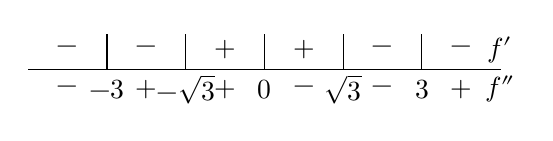
\begin{tikzpicture}[yscale=1]
            \draw (0, 0)--(6, 0);
            \foreach \x/\y in {-3/1, -\sqrt{3}/2, 0/3, \sqrt{3}/4, 3/5}{
              \node at (\y, -0.25) {$\x$};
              \draw[xshift=\y cm] (0, 0) -- (0, 0.45);}
              \foreach \x/\y in {0/$-$, 1/$-$, 2/$+$, 3/$+$, 4/$-$, 5/$-$}
              \node at (\x + 0.5, 0.25) {\y};
              \foreach \x/\y in {0/$-$, 1/$+$, 2/$+$, 3/$-$, 4/$-$, 5/$+$}
              \node at (\x + 0.5, -0.25) {\y};
            \node at (6, -0.25) {$f''$};
            \node at (6, 0.25) {$f'$};
          \end{tikzpicture}
        }
        \end{center}
        \vfill\item \onslide<+->{interval of increase: }\onslide<+->{ interval that $f' > 0$. }\onslide<+->{ $(-\sqrt{3}, \sqrt{3})$.}
        \vfill\item \onslide<+->{interval of decrease: }\onslide<+->{ interval that $f' < 0$. }\onslide<+->{ $(-\infty, -\sqrt{3})$ or $(\sqrt{3}, \infty)$.}
        \vfill\item \onslide<+->{critical points: }\onslide<+->{ $f' = 0$. }\onslide<+->{ $x = \pm\sqrt{3}$.}
        \vfill\item \onslide<+->{concavity: }\onslide<+->{ intervals that $f'' > 0$ concave up, $\,\,f'' < 0$ concave down. }
        \vfill\item \onslide<+->{inflection points: }\onslide<+->{ $f'' = 0$ and of different sign before and after. }\onslide<+->{ $x = -3, 0, 3$.}
        \vfill\item \onslide<+->{Sketch the graph:}
        \onslide<+->{
        \begin{center}
          \sageplot[width=4cm]{plot(x / (x^2 + 3), -5, 5)}
        \end{center}
      }
      \end{itemize}

  \end{itemize}
\end{frame}

\begin{frame}[fragile]
  \frametitle{Example II}
  \begin{itemize}
      \item\onslide<+->{Determine the intervals of increase and decrease, the local extreme values, the concavity and the graph of $f(x) = x^4 - 2 x^3 + 1$.}
      \begin{itemize}
        \vfill\item \onslide<+->{$f'(x) = 4 x^3 - 6 x^2 = 4 x^2(x - \frac{3}{2})$, }\onslide<+->{ $f''(x) = 12 x^2 - 12 x = 12x(x - 1)$.}
        \vfill\item \onslide<+->{List the critical and inflection points and decide the sign of $f'$, $f''$ in each interval:}
        \begin{center}
          \onslide<+->{
          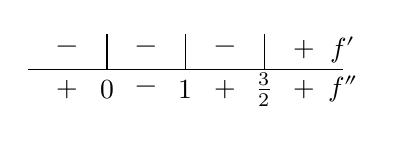
\begin{tikzpicture}[yscale=1]
            \draw (0, 0)--(4, 0);
            \foreach \x/\y in {0/1, 1/2, \frac{3}{2}/3}{
              \node at (\y, -0.25) {$\x$};
              \draw[xshift=\y cm] (0, 0) -- (0, 0.45);}
            \foreach \x/\y in {0/$-$, 1/$-$, 2/$-$, 3/$+$}
              \node at (\x + 0.5, 0.25) {\y};
            \foreach \x/\y in {0/$+$, 1/$-$, 2/$+$, 3/$+$}
              \node at (\x + 0.5, -0.25) {\y};
            \node at (4, -0.25) {$f''$};
            \node at (4, 0.25) {$f'$};
          \end{tikzpicture}
        }
        \end{center}
        \vfill\item \onslide<+->{critical points: }\onslide<+->{ $f' = 0$. }\onslide<+->{ $x = 0, \frac{3}{2}$.}
        \vfill\item \onslide<+->{interval of increase: }\onslide<+->{ interval that $f' > 0$. }\onslide<+->{ $(\frac{3}{2}, \infty)$.}
        \vfill\item \onslide<+->{interval of decrease: }\onslide<+->{ interval that $f' < 0$. }\onslide<+->{ $(-\infty, \frac{3}{2})$.}
        \vfill\item \onslide<+->{inflection points: }\onslide<+->{ $f'' = 0$ and of different sign before and after. }\onslide<+->{ $x = 0, 1$.}
        \vfill\item \onslide<+->{Sketch the graph:}
        \onslide<+->{
        \begin{center}
          \sageplot[width=4cm]{plot(x^4 - 2 * x^3 + 1, -1.2, 2.1)}
        \end{center}
      }
      \end{itemize}
      
  \end{itemize}
\end{frame}

\begin{frame}[fragile]
  \frametitle{Example III}
  \begin{itemize}
    \item\onslide<+->{Determine the intervals of increase and decrease, the local extreme values, the concavity and the graph of $f(x) = \frac{x^3}{x^2 - 1}$.}
      \begin{itemize}
          \vfill\item \onslide<+->{$f'(x) = \frac{x^2(x^2 - 3)}{(x^2 -1)^2} = \frac{x^2(x - \sqrt{3})(x + \sqrt{3})}{(x^2 -1)^2}$, }\onslide<+->{ $f''(x) = \frac{2x(x^2 + 3)}{(x^2 - 1)^3}$.}
          \vfill\item \onslide<+->{List the critical, singular, and inflection points and decide the sign of $f'$, $f''$ in each interval:}
        \begin{center}
          \onslide<+->{
          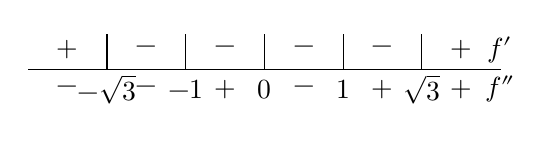
\begin{tikzpicture}[yscale=1]
            \draw (0, 0)--(6, 0);
            \foreach \x/\y in {-\sqrt{3}/1, -1/2, 0/3, 1/4, \sqrt{3}/5}{
              \node at (\y, -0.25) {$\x$};
              \draw[xshift=\y cm] (0, 0) -- (0, 0.45);}
            \foreach \x/\y in {0/$+$, 1/$-$, 2/$-$, 3/$-$, 4/$-$, 5/$+$}
              \node at (\x + 0.5, 0.25) {\y};
            \foreach \x/\y in {0/$-$, 1/$-$, 2/$+$, 3/$-$, 4/$+$, 5/$+$}
              \node at (\x + 0.5, -0.25) {\y};
            \node at (6, -0.25) {$f''$};
            \node at (6, 0.25) {$f'$};
          \end{tikzpicture}
        }
        \end{center}
        \vfill\item \onslide<+->{singular points: }\onslide<+->{ $x^2 - 1 = 0$. }\onslide<+->{ vertical asymptotes $x = \pm1$.}
        \vfill\item \onslide<+->{asympote: }\onslide<+->{ $y = x$, }\onslide<+->{ for $\lim_{x\to\pm\infty}\big(\frac{x^3}{x^2 - 1} - x\big) = 0$}
        \vfill\item \onslide<+->{critical points: }\onslide<+->{ $f' = 0$. }\onslide<+->{ $x = 0, \pm\sqrt{3}$.}
        \vfill\item \onslide<+->{interval of increase: }\onslide<+->{ interval that $f' > 0$. }\onslide<+->{ $(-\infty, -\sqrt{3})$ or $(\sqrt{3}, \infty)$.}
        \vfill\item \onslide<+->{interval of decrease: }\onslide<+->{ interval that $f' < 0$. }\onslide<+->{ $(-\sqrt{3}, \sqrt{3})$.}
        \vfill\item \onslide<+->{Sketch the graph:}
        \onslide<+->{
        \begin{center}
          \sageplot[width=4cm]{plot(x^3 / (x^2 - 1), -5, 5, ymin=-5, ymax=5)}
        \end{center}
      }
      \end{itemize}
      
  \end{itemize}
\end{frame}

\section{Extreme-Value Problems}

\begin{frame}[fragile]
  \frametitle{Example I}
  \begin{columns}
    \begin{column}{0.25\textwidth}
      \onslide<+->{\begin{center}\includegraphics[width=\textwidth]{./figures/applications/extra/line_dist.pdf}\end{center}}
    \end{column}
    \begin{column}{0.75\textwidth}
      \begin{itemize}
        \item Find the point on the line $y=6-3x$ that is closest to $(7, 5)$ and the shortest distance.
        \vfill\item
        \vfill\item \hyperlink{thm:opt}{\beamerbutton{Review of the Key Theorem}}
      \end{itemize}
    \end{column}
  \end{columns}

  \begin{itemize}
    \vfill\item\onslide<+->{Let $\ell$ be the distance from the point $(x, y)$ on line $y = 6-3x$ to the point $(7, 5)$, then}
      \begin{align*}
        \onslide<+->{\ell^2 = (x-7)^2 + (y-5)^2 = (x-7)^2 + (6-3x-5)^2 = 10(x^2-2x+5)} 
      \end{align*}
    \vfill\item\onslide<+->{\hypertarget{app}{As $x \to \pm \infty$, $\ell\to +\infty$, and $\ell(0)=5\sqrt{2} < \infty$, so the absolute minimum exists.}} 
    \vfill\item\onslide<+->{To minimize $\ell$ is equivalent to minimize $\ell^2$.}
    \vfill\item\onslide<+->{Compute the derivative of $\ell^2(x)$:}
      \begin{align*}
        \onslide<+->{(\ell^2(x))' &= 10(2x - 2)} 
      \end{align*}
    \vfill\item\onslide<+->{The minimizer $x^\star$ is the root of $(\ell^2(x))' = 0$, i.e. $x^\star = 1$.}
    \vfill\item\onslide<+->{The minimal distance is $\ell(1) = 2\sqrt{10}$ and occurs at $x=1$, $y = 6 - 3 = 3$.}
  \end{itemize}
\end{frame}

\begin{frame}[fragile]
  \frametitle{Example II}
  \begin{columns}
    \begin{column}{0.25\textwidth}
      \onslide<+->{\begin{center}
\includegraphics[width=\textwidth]{./figures/applications/hyperbolaMaxMin.pdf}\end{center}}
    \end{column}
    \begin{column}{0.75\textwidth}
      Find the point on $y^2 = x^2 + 1$ that is closest to $(2, 0)$ and the shortest distance.
    \end{column}
  \end{columns}

  \begin{itemize}
    \item\onslide<+->{Let $\ell$ be the distance from the point $(x, y)$ on $y^2 = x^2 + 1$ to the point $(2, 0)$, then}
      \begin{align*}
        \onslide<+->{\ell^2 = (x-2)^2 + (y-0)^2 = (x-2)^2 + (x^2 + 1) = 2 x^2 - 4x + 5} 
      \end{align*}
    \vfill\item\onslide<+->{As $x\to\pm\infty$, $\ell\to +\infty$, and $\ell(0)=\sqrt{5} < \infty$, so the absolute minimum exists.} 
    \vfill\item\onslide<+->{To minimize $\ell$ is equivalent to minimize $\ell^2$.}
    \vfill\item\onslide<+->{Compute the derivative of $\ell^2(x)$:}
      \begin{align*}
        \onslide<+->{(\ell^2(x))' &= 4x - 4} 
      \end{align*}
    \vfill\item\onslide<+->{The minimizer $x^\star$ is the root of $(\ell^2(x))' = 0$, i.e. $x^\star = 1$.}
    \vfill\item\onslide<+->{The minimal distance is $\ell(1) = \sqrt{3}$ and occurs at $x=1$, $y = \pm\sqrt{2}$.}
  \end{itemize}
\end{frame}

\begin{frame}
  \frametitle{Example III}
  \begin{columns}
    \begin{column}{0.55\textwidth}
      \onslide<+->{\begin{center}\includegraphics[scale=.5]{./figures/applications/inscribedB.pdf}\quad\includegraphics[scale=.5]{./figures/applications/inscribed.pdf}\end{center}}
    \end{column}
    \begin{column}{0.45\textwidth}
      \begin{itemize}
        \item Find the dimensions of the rectangle of largest area that can be inscribed in an equilateral triangle of side $a$ if one side of the rectangle lies on the base of the triangle.
      \end{itemize}
    \end{column}
  \end{columns}
  \begin{itemize}
    \item\onslide<+->{Let $(x, y)$ be a point on the line that connects $(0, \frac{\sqrt{3}}{2}a)$ and $(\frac{a}{2}, 0)$.} 
    \vfill\item\onslide<+->{The line that connects $(0, \frac{\sqrt{3}}{2}a)$ and $(\frac{a}{2}, 0)$ is }\onslide<+->{$y = -\sqrt{3}x + \frac{\sqrt{3}}{2}a$.}
    \vfill\item\onslide<+->{The area of the inscribed rectangle $A = 2xy$; }\onslide<+->{ substitute $y = -\sqrt{3}x + \frac{\sqrt{3}}{2}a$, }\onslide<+->{ the area of the rectangle $A(x) = 2x\Big(-\sqrt{3}x + \frac{\sqrt{3}}{2}a\Big) = \sqrt{3} x(a - 2x)$, }\onslide<+->{ where $0\leqslant x\leqslant\frac{a}{2}$.}
    \vfill\item\onslide<+->{As $x=0, \frac{a}{2}$, $A(x)=0$, and $A(\frac{a}{10}) > 0$, so the absolute maximum exists.} 
    \vfill\item\onslide<+->{Compute the derivative of $A(x)$:
      \begin{align*}
        \onslide<+->{A'(x) = \sqrt{3} \big( x \cdot (-2) + 1 \cdot (a-2x) \big) = \sqrt{3}(a-4x)}
      \end{align*}
      \onslide<+->{The minimizer $x^\star$ is the root of $A'(x) = 0$, i.e. $x^\star = \frac{a}{4}$.}
    }
    \vfill\item\onslide<+->{The largest such rectangle has dimensions $2\times\frac{a}{4} = \frac{a}{2}$ by $-\sqrt{3}\,\frac{a}{4} + \frac{\sqrt{3}}{2}a=\frac{\sqrt{3}}{4}a$.}
  \end{itemize}
\end{frame}

\begin{frame}
  \frametitle{Example IV}
  \begin{columns}
    \begin{column}{0.55\textwidth}
      \onslide<+->{\begin{center}\includegraphics[scale=.5]{./figures/applications/extra/gutter.pdf}\end{center}}
    \end{column}
    \begin{column}{0.45\textwidth}
      \begin{itemize}
        \item A water trough is to be constructed from a metal sheet of width $45$ cm by bending up one third of the sheet on each side through an angle $\theta$.  Which $\theta$ will allow the trough to carry the maximum amount of water?
      \end{itemize}
    \end{column}
  \end{columns}
  \begin{itemize}
    \item\onslide<+->{The problem amounts to maximize the cross-sectional area $A$.} 
      \vfill\item\onslide<+->{$A(\theta) = \frac{1}{2}\times 15\sin\theta\cdot 15\cos\theta\times 2 $}\onslide<+->{ $ + 15\times 15\sin\theta$}\onslide<+->{ $= 225\sin\theta(\cos\theta + 1)$, }\onslide<+->{ where $0\leqslant\theta\leqslant\pi$.}
    \vfill\item\onslide<+->{As $\theta=0, \pi$, $A(\theta)=0$, and $A(\frac{\pi}{2}) = 225 > 0$, so the absolute maximum exists.} 
    \vfill\item\onslide<+->{Compute the derivative of $A(\theta)$:}
      \begin{align*}
        \onslide<+->{A'(\theta) = 225 \cos\theta \cdot (1+\cos\theta) + 225 \sin\theta \cdot(-\sin\theta)}\onslide<+->{= 225 (\cos\theta +2\cos^2\theta -1)}
      \end{align*}
      \onslide<+->{The minimizer $\theta^\star$ is the root of $A'(\theta) = 0$, i.e. $\cos\theta^\star +2\cos^2\theta^\star -1$ $= (2\cos\theta^\star - 1)(\cos \theta^\star + 1) = 0$, }\onslide<+->{ For $0 < \theta^\star < \pi$, $2\cos\theta^\star-1 = 0$, so $\theta^\star = \frac{\pi}{3}$.}
    \vfill\item\onslide<+->{The largest area $A(\frac{\pi}{3}) = 225\sin(\frac{\pi}{3})(\cos(\frac{\pi}{3}) + 1) = 225\cdot\frac{3\sqrt{3}}{4}\approx 292.28$.}
  \end{itemize}
\end{frame}

\begin{frame}[fragile]
  \frametitle{Example V}
  \begin{columns}
    \begin{column}{0.35\textwidth}
      \onslide<+->{\begin{center}
\includegraphics[width=\textwidth]{./figures/applications/snell.pdf}\end{center}}
    \end{column}
    \begin{column}{0.65\textwidth}
      The Fermat principle states that the path of light travels from $P$ to $Q$ takes minimal time; establish the Snell's law $\frac{\sin\theta_i}{\sin\theta_r} = \frac{c_a}{c_w}$, where $c_a$, $c_w$ be the speed of light in air and water.
      \onslide<+->{\begin{center}
\includegraphics[width=0.6\textwidth]{./figures/applications/snellB.pdf}\end{center}}
    \end{column}
  \end{columns}
  \begin{itemize}
    \item \onslide<+->{Denote the total travel time of the light from $P$ to $Q$ by $T$, then }
    \begin{align*}
      \onslide<+->{T(x) &= \frac{1}{c_a}\sqrt{(X_P-x)^2+Y_P^2} + \frac{1}{c_w}\sqrt{(X_Q-x)^2+Y_Q^2}}
    \end{align*}
    \onslide<+->{As $x\to\pm\infty$, $T\to\infty$, and $T(0) = \frac{\sqrt{X_P^2+Y_P^2}}{c_a} + \frac{\sqrt{X_Q^2+Y_Q^2}}{c_w} < \infty$, so the absolute minimum exists.}
    \vfill\item\onslide<+->{The critical point $x^\star$ satisfies $T'(x^\star) = 0$, i.e. }
    \begin{align*}
      \onslide<+->{0 &= \frac{1}{c_a} \frac{X_P-x^\star}{\sqrt{(X_P-x^\star)^2+Y_P^2}} + \frac{1}{c_w} \frac{X_Q-x^\star}{\sqrt{(X_Q-x^\star)^2+Y_Q^2}} }\onslide<+->{ = \frac{-\sin\theta_i}{c_a} + \frac{\sin\theta_r}{c_w}}\onslide<+->{\,\,\Longrightarrow\,\,\frac{\sin\theta_i}{\sin\theta_r}=\frac{c_a}{c_w}}
    \end{align*}
  \end{itemize}
\end{frame}

\begin{frame}
  \frametitle{Example VI}
  \begin{columns}
    \begin{column}{0.55\textwidth}
      \onslide<+->{\begin{center}
\includegraphics[width=\textwidth]{./figures/applications/extra/corridor.pdf}\end{center}}
    \end{column}
    \begin{column}{0.45\textwidth}
      \begin{itemize}
        \item Find the length of the longest rod that can be carried horizontally (no tilting allowed) from a corridor $3$m wide into a corridor $2$m wide.
      \end{itemize}
    \end{column}
  \end{columns}
  \begin{itemize}
    \item\onslide<+->{Suppose that the angle between the rod and the inner wall of the $3$m corridor is $\theta$, then the total length of the rod is} 
      \begin{align*}
        \onslide<+->{\ell(\theta) = \ell_1(\theta) +\ell_2(\theta) = \frac{3}{\sin\theta}+\frac{2}{\cos\theta}\qquad 0\leqslant\theta\leqslant\frac{\pi}{2}}
      \end{align*}
    \vfill\item\onslide<+->{The length of the longest rod one can move through the corridor is the minimum of $\ell(\theta)$.}
    \vfill\item\onslide<+->{As $\theta \to 0+, \frac{\pi}{2}-$, $\ell(\theta)\to+\infty$, and $\ell(\frac{\pi}{4})=5\sqrt{2} < \infty$, so $\ell(\theta)$ has an absolute minimum.} 
    \vfill\item\onslide<+->{Find $\theta^\star$, the root of $\ell'(\theta) = 0$:} 
      \begin{align*}
        \onslide<+->{\ell'(\theta) &= -\frac{3 \cos\theta}{\sin^2\theta} + \frac{2\sin\theta}{\cos^2\theta} = \frac{-3\cos^3\theta +2 \sin^3\theta}{\sin^2\theta\cos^2\theta} = 0\,\,\Longrightarrow\,\,\tan\theta^\star = \sqrt[3]{\frac{3}{2}}}
      \end{align*}
    \item \onslide<+->{Substituting $\theta^\star$ we find the minimum of $\ell$:}
      \begin{align*}
        \onslide<+->{\ell(\theta^\star) = \frac{3}{\sin\theta^\star} + \frac{2}{\cos\theta^\star}}\onslide<+->{=\frac{3}{\frac{\root 3\of 3}{\sqrt{2^{\nicefrac{2}{3}}+3^{\nicefrac{2}{3}}}}} +\frac{2}{\frac{\root 3\of 2}{\sqrt{2^{\nicefrac{2}{3}}+3^{\nicefrac{2}{3}}}} }}\onslide<+->{ = {\big(2^{\nicefrac{2}{3}}+3^{\nicefrac{2}{3}}\big)}^{\nicefrac{3}{2}}\approx 7.02 \text{m}}
      \end{align*}
  \end{itemize}
\end{frame}

\section{Linear Approximations, Taylor Polynomials}

\begin{frame}
  \frametitle{Taylor's Theorem}
  \begin{itemize}
    \item\onslide<+->{Let $f$ be defined on an open interval $I$, $a, b\in I$, }\onslide<+->{ and $f^{(n+1)}$ exists on $I$, $n\in\mathbb{Z}^+$.} 
    \vfill\item\onslide<+->{Then $\exists\,c$ lies between $a$ and $b$ s.t. }
      \begin{align*}
        \onslide<+->{f(b) = f(a) + f'(a)(b - a) + \frac{f''(a)}{2!}(b - a)^2 +\cdots+\frac{f^{(n)}(a)}{n!}(b-a)^n + \frac{f^{(n+1)}(c)}{(n + 1)!}(b-a)^{n+1}}
      \end{align*}
  \end{itemize}
  
  \color{C2}
  \begin{itemize}
    \item\onslide<+->{Since differentiability implies continuity, $f$, $f'$, $f''$, $\ldots$, $f^{(n)}$ are all continuous on $I$.} 
    \vfill\item\onslide<+->{WLOG, let $a < b$.}
    \vfill\item\onslide<+->{Let $M$, $g(t)$ be defined s.t.}
      \begin{align*}
        \onslide<+->{f(b) &= f(a) + f'(a)(b - a) + \frac{f''(a)}{2!}(b - a)^2 +\cdots+\frac{f^{(n)}(a)}{n!}(b-a)^n + \frac{M}{(n + 1)!}(b-a)^{n+1}\\}
        \onslide<+->{g(t) &= -f(b) + f(t) + f'(t)(b - t) + \frac{f''(t)}{2!}(b - t)^2 +\cdots+\frac{f^{(n)}(t)}{n!}(b-t)^n + \frac{M}{(n + 1)!}(b-t)^{n+1}}
      \end{align*}
    \vfill\item\onslide<+->{Note that $g(a) = 0$, $g(b) = 0$, then by Rolle's Theorem, $\exists\,c\in(a, b)$ s.t. $g'(c) = 0$.}
      \begin{align*}
        \onslide<+->{g'(t) &= f'(t) - f'(t) + f''(t)(b-t) - f''(t)(b-t) + \frac{f'''(t)}{2!}(b - t)^2 -+ \cdots\\}
        \onslide<+->{      &=  \frac{f^{(n+1)}(t) - M}{n!}(b-t)^n}
      \end{align*}
    \vfill\item\onslide<+->{So $g'(c) = 0$ implies $f^{(n+1)}(c) - M = 0\,\,\Longrightarrow\,\, M = f^{(n+1)}(c)$.}
  \end{itemize}
\end{frame}

\begin{frame}
  \frametitle{Taylor/Maclaurin Polynomials, Linear Approximation/Linearization}
  \begin{itemize}
    \item\onslide<+->{Let $f$ be defined on an open interval $I$, $a, x\in I$, }\onslide<+->{ and $f^{(n+1)}$ exists on $I$, $n\in\mathbb{Z}^+$.} 
      \vfill\item\onslide<+->{The $n$-th order Taylor polynomial $P_n(x)$ for $f$ about $x = a$ is defined as}
      \begin{align*}
        \onslide<+->{P_n(x) = f(a) + f'(a)(x - a) + \frac{f''(a)}{2!}(x - a)^2 +\cdots+\frac{f^{(n)}(a)}{n!}(x-a)^n}
      \end{align*}
    \vfill\item\onslide<+->{The $n$-th order Taylor polynomial $P_n(x)$ for $f$ about $x = 0$ is also called the Maclaurin polynomial.}
    \vfill\item\onslide<+->{$P_1(x)$ for $f$ about $x = a$ is called the linearization of $f$ near $x = a$.}

    \color{C2}
    \vfill\item\onslide<+->{Example: $P_2(x)$ for $f(x) = \sqrt{x}$ about $x = 25$ is }\onslide<+->{ $5 + \frac{1}{10}(x - 25) - \frac{1}{1000}(x - 25)^2$}
    \vfill\item\onslide<+->{Example: $P_3(x)$ for $f(x) = \ln{x}$ about $x = e$ is }\onslide<+->{ $1 + \frac{1}{e}(x - e) - \frac{1}{2e^2}(x - e)^2 + \frac{1}{3e^3}(x - e)^3$}
    \vfill\item\onslide<+->{Example: the Maclaurin polynomial of order $6$ for $\exp$ is }\onslide<+->{ $1 + x + \frac{x^2}{2!} + \frac{x^3}{3!} + \frac{x^4}{4!} + \frac{x^5}{5!} + \frac{x^6}{6!}$}
    \vfill\item\onslide<+->{Example: the Maclaurin polynomial of order $9$ for $\sin$ is }\onslide<+->{ $x - \frac{x^3}{3!} + \frac{x^5}{5!} - \frac{x^7}{7!} + \frac{x^9}{9!}$}
    \vfill\item\onslide<+->{Example: the Maclaurin polynomial of order $8$ for $\cos$ is }\onslide<+->{ $1 - \frac{x^2}{2!} + \frac{x^4}{4!} - \frac{x^6}{6!} + \frac{x^8}{8!}$}
    \vfill\item\onslide<+->{Example: the Maclaurin polynomial of order $6$ for $\frac{1}{1-x}$ is }\onslide<+->{ $1 + x + x^2 + x^3 + x^4 + x^5 + x^6$}
    \vfill\item\onslide<+->{Example: the Maclaurin polynomial of order $5$ for $\ln(1+x)$ is }\onslide<+->{ $x - \frac{x^2}{2} + \frac{x^3}{3} - \frac{x^4}{4} + \frac{x^5}{5}$}
  \end{itemize}
\end{frame}

\begin{frame}
  \frametitle{Maclaurin Polynomial Approximation of Cosine}
    \begin{center}
      \onslide<+->{\includegraphics[scale=.5]{./figures/approx1d.pdf}}
      \qquad
      \onslide<+->{\includegraphics[scale=.5]{./figures/approx2d.pdf}}
    \end{center}
    \begin{center}
      \onslide<+->{\includegraphics[scale=.5]{./figures/approx3d.pdf}}
      \qquad
      \onslide<+->{\includegraphics[scale=.5]{./figures/approx4d.pdf}}
    \end{center}
\end{frame}

\begin{frame}
  \frametitle{Maclaurin Polynomial Approximation of Sine}
    \begin{center}
      \onslide<+->{\includegraphics[scale=.5]{./figures/approx1c.pdf}}
      \qquad
      \onslide<+->{\includegraphics[scale=.5]{./figures/approx2c.pdf}}
    \end{center}
    \begin{center}
      \onslide<+->{\includegraphics[scale=.5]{./figures/approx3c.pdf}}
      \qquad
      \onslide<+->{\includegraphics[scale=.5]{./figures/approx4c.pdf}}
    \end{center}
\end{frame}

%%%%%%%%%%%%%%%%%%%%%%%%% render boundary
%}{}

\section{Ideas of Integration}

\begin{sagesilent}
def RiemannRec(a, b, n, f):
    t = var('t')
    delta = (b - a) / n
    LowerY = find_local_minimum(f, a, b)[0] - .5
    UpperY = find_local_maximum(f, a, b)[0] + .5
    step = .01
    x_coords = [t for t in srange(a, b, step)]
    y_coords = [f(t).n(digits=4) for t in srange(a, b, step)]
####################### Picture
    output = r"\begin{tikzpicture}[scale=0.9]"
    output += r"\begin{axis}["
    output += r"xtick=\empty, ytick=\empty,"
    output += r"grid = none,"
    output += r"thick,black,"
    output += r"scale=1,"
    output += r"axis lines=center,"
    output += r"line join=bevel,"
    output += r"xmin=%f, xmax=%f, ymin=%f, ymax=%f]" % (a -.5, b + .5, LowerY, UpperY)
#### Left hand rectangles
    for i in range(0, n):
        output += r"\draw[color=Red, pattern=north west lines, pattern color=Red!90, opacity=.4]  (%s, 0) rectangle (%s, %s); "% (a + i* delta, a + (i + 1) * delta, f(a + i * delta))
#### Right hand rectangles
    for i in range(0, n):
        output += r"\draw[color=NavyBlue, pattern=north east lines, pattern color=NavyBlue!90!white, opacity=.4] (%s, 0) rectangle (%s, %s);" % (a + i * delta, a + (i + 1) * delta, f(a + (i + 1) * delta))
####### the function
    output += r"\addplot[smooth] coordinates {"
    for i in range(0, len(x_coords) - 1):
        output += r"(%s, %s)" % (x_coords[i], y_coords[i])
    output += r"};"
#### a and b
    output += r"\draw[dashed] (%s, 0)--(%s, 1) node[above] {$a$};" % (a, a)
    output += r"\draw[dashed] (%s, 0)--(%s, -1) node[below] {$b$};" % (b, b)
    output += r""
    output += r"\end{axis}"
    output += r"\end{tikzpicture}"

    return output

f(x) = (sin(x^2) + 2).function(x)
fig1 = RiemannRec(1.0, 3.0, 20, f) #a,b,n,function
\end{sagesilent}

\begin{frame}[fragile]
  \frametitle{Definition of the (Riemann) Integral}
  \begin{center}
    \onslide<+->{
    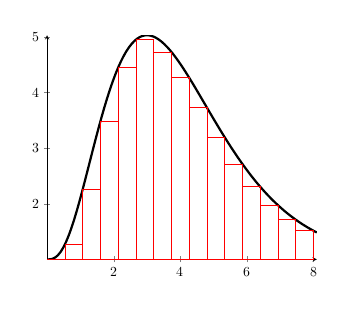
\begin{tikzpicture}[scale=0.5]
      \pgfset{declare function={f(\x)=3*exp(-(\x))*(\x)^3+1;}}
      \begin{axis}[domain=0:8.1,
          samples=100,
          axis lines=middle
      ]
      \addplot [ultra thick] {f(x)};
      \addplot [red,
        integral segments=15,
        integral min=0:8
      ] {f(x)};
    \end{axis}
  \end{tikzpicture}
}
  \qquad
    \onslide<+->{
  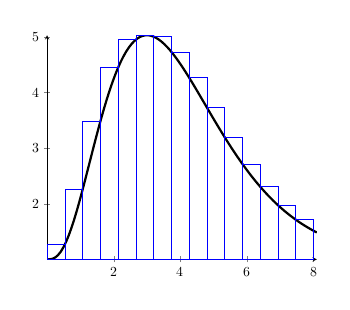
\begin{tikzpicture}[scale=0.5]
  \pgfset{declare function={f(\x)=3*exp(-(\x))*(\x)^3+1;}}
  \begin{axis}[
      domain=0:8.1,
      samples=100,
      axis lines=middle
  ]
  \addplot [ultra thick] {f(x)};

  \addplot [
      blue,
      integral segments=15,
      integral max=0:8
  ] {f(x)};
  \end{axis}
  \end{tikzpicture}
}
  \end{center}

  \begin{itemize}
    \item\onslide<+->{Let $f:[a,b]\mapsto\mathbb{R}$ be continuous, $\mathbb{P}: a = x_0 < x_1 < x_2 < \cdots < x_n = b$ be a partition of $[a, b]$.}
    \vfill\item\onslide<+->{Let $\Delta_k=x_k - x_{k-1}$, $\|\mathbb{P}\| = \max\{\left|\Delta_k\right|: 1\leqslant k\leqslant n\}$, $x_{k-1}\leqslant t_k \leqslant x_k$, $k=1,2,\ldots,n$.}
    \vfill\item\onslide<+->{Let $f_k = f(t_k)$, $u_k = \sup\left\{f(x): x_{k-1}\leqslant x\leqslant x_k\right\}$, $l_k = \inf\left\{f(x): x_{k-1}\leqslant x\leqslant x_k\right\}$, $k=1,2,\ldots,n$.}
    \vfill\item\onslide<+->{Define the sums }\onslide<+->{ $R(f,\mathbb{P}) = \sum_{k=1}^n f_k\,\Delta_k$, }\onslide<+->{ $U(f,\mathbb{P}) = \sum_{k=1}^n u_k\,\Delta_k$, } \onslide<+->{ $L(f,\mathbb{P}) = \sum_{k=1}^n l_k\,\Delta_k$.}
    \vfill\item\onslide<+->{A priori $L(f,\mathbb{P})\leqslant R(f,\mathbb{P})\leqslant U(f, \mathbb{P})$; Define 
      \begin{align*}
        \int_a^b f(x)\,\mathrm{d}x = \lim_{\substack{n\to\infty \\ \|\mathbb{P}\|\to 0}} R(f,\mathbb{P}) 
      \end{align*}
    }
  \end{itemize}

  \ifbool{integral}{
  \begin{center}
    \onslide<+->{
    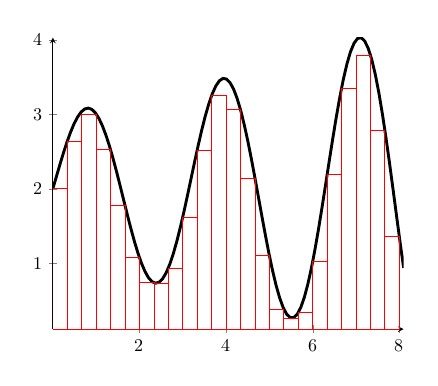
\begin{tikzpicture}[scale=0.65]  
      \pgfset{declare function={f(\x)=sin(2*deg(\x))*exp(0.1*\x)+2;}}
      \begin{axis}[
        domain=0:8.1,
        samples=100,
        axis lines=middle
      ]
      \addplot [ultra thick] {f(x)};

      \addplot [red,
        integral segments=24,
        integral min=0:8
      ] {f(x)};
    \end{axis}
  \end{tikzpicture}
}
  \qquad
  \onslide<+->{
  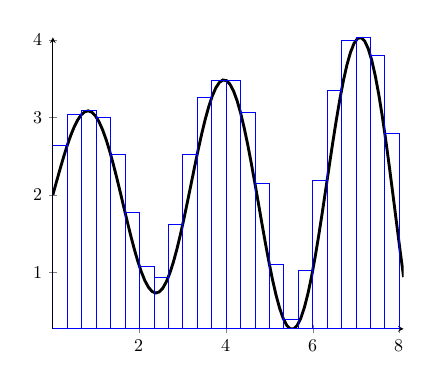
\begin{tikzpicture}[scale=0.65] 
  \pgfset{declare function={f(\x)=sin(2*deg(\x))*exp(0.1*\x)+2;}}
  \begin{axis}[
      domain=0:8.1,
      samples=100,
      axis lines=middle
  ]
  \addplot [ultra thick] {f(x)};

  \addplot [
      blue,
      integral segments=24,
      integral max=0:8,
  ] {f(x)};
  \end{axis}
  \end{tikzpicture}
}
\end{center}

  \begin{center}
    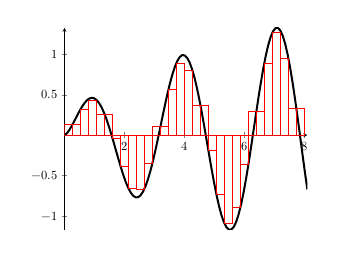
\begin{tikzpicture}[scale=0.45]
      \pgfset{declare function={f(\x)=sqrt(\x)*cos(deg(\x))*sin(deg(\x));}}
      \begin{axis}[
          domain=0:8.1,
          samples=100,
          axis lines=middle
       ]
    \addplot [ultra thick] {f(x)};

  \addplot [
      red,
      integral segments=30,
      integral min=0:8
  ] {f(x)};
  \end{axis}
  \end{tikzpicture}
  \qquad
  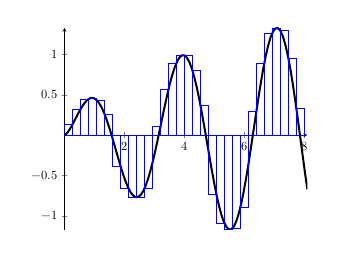
\begin{tikzpicture}[scale=0.45] 
  \pgfset{declare function={f(\x)=sqrt(\x)*cos(deg(\x))*sin(deg(\x));}}
  \begin{axis}[
      domain=0:8.1,
      samples=100,
      axis lines=middle
  ]
  \addplot [,ultra thick] {f(x)};

  \addplot [
      blue,
      integral segments=30,
      integral max=0:8
  ] {1};
  \end{axis}
  \end{tikzpicture}

  \sagestr{fig1}
  \end{center}
}{}
\end{frame}

\begin{frame}
  \frametitle{Properties of the Integral}
  \begin{itemize}
    \item\onslide<+->{Let $f$, $g$ be integrable on an interval containing $a$, $b$, $c$, and constants $\alpha$, $\beta$. Then} 
      \begin{align*}
        \onslide<+->{\int_a^a f(x)\,\mathrm{d}x &= 0\\}
        \onslide<+->{\int_a^b f(x)\,\mathrm{d}x &= -\int_b^a f(x)\,\mathrm{d}x\\}
        \onslide<+->{\int_a^b \big(\alpha\,f(x) + \beta\,g(x)\big)\,\mathrm{d}x &= \alpha\int_a^b f(x)\,\mathrm{d}x + \beta\int_a^b g(x)\,\mathrm{d}x\\}
        \onslide<+->{\int_a^b f(x)\,\mathrm{d}x + \int_b^c f(x)\,\mathrm{d}x &= \int_a^c f(x)\,\mathrm{d}x\\}
        \onslide<+->{\int_a^b f(x)\,\mathrm{d}x &\leqslant \int_a^b g(x)\,\mathrm{d}x,\quad\text{ if }\,\,f(x)\leqslant g(x)\,\text{ on }\,[a, b],\,\,a\leqslant b. \\}
        \onslide<+->{\left|\,\int_a^b f(x)\,\mathrm{d}x\,\right| &\leqslant \int_a^b \left|\,f(x)\,\right|\,\mathrm{d}x, \quad a\leqslant b. \\}
        \onslide<+->{\int_{-a}^a f(x)\,\mathrm{d}x &= 0, \qquad\text{ if $\,f(x)\,$ is odd.}\\}
        \onslide<+->{\int_{-a}^a f(x)\,\mathrm{d}x &= 2\int_0^a f(x)\,\mathrm{d}x, \quad\text{ if $\,f(x)\,$ is even.}\\}
      \end{align*}
  \end{itemize}
\end{frame}

\begin{frame}
  \frametitle{Properties of the Integral: Examples}
  \begin{itemize}
    \item\onslide<+->{Interpreting integrals as areas and using the properties of the integral:} 
      \begin{align*}
        \onslide<+->{\int_{-\sqrt{2}}^{\sqrt{2}} \sqrt{2 - x^2}\,\mathrm{d}x &= }\onslide<+->{ \pi\quad\text{(The area of the upper circle of radius $\sqrt{2}$)}\\}
        \onslide<+->{\int_{-1}^2 \sgn(x)\,\mathrm{d}x = }\onslide<+->{2\cdot 1 - 1\cdot 1 &= }\onslide<+->{ 1\quad\text{(the difference of two rectangles)}\\}
        \onslide<+->{\int_{-\pi}^{\pi} \sin(x^7-5x^3)\,\mathrm{d}x &= }\onslide<+->{ 0\quad\text{($\sin(x^7-5x^3)$ is odd)}\\}
        \onslide<+->{\int_{-6}^{6} e^{-x^4}\sin(\sin x)\,\mathrm{d}x &= }\onslide<+->{ 0\quad\text{($e^{-x^4}\sin(\sin x)$ is odd)}\\}
        \onslide<+->{\int_{-4}^{4} \big(e^{x} - e^{-x}\big)\,\mathrm{d}x &= }\onslide<+->{ 0\quad\text{($e^{x} - e^{-x}$ is odd)}\\}
        \onslide<+->{\int_{-100}^{100} \big(e^{9x^5-2x^7} - e^{-9x^5 + 2x^7}\big)\,\mathrm{d}x &= }\onslide<+->{ 0\quad\text{($e^{9x^5-2x^7} - e^{-9x^5 + 2x^7}$ is odd)}\\}
        \onslide<+->{\int_{-a}^a |x|\,\mathrm{d}x = }\onslide<+->{2\int_0^a |x|\,\mathrm{d}x &= }\onslide<+->{ a^2\quad\text{($|x|$ is even; area of two $a\times a$ triangles)}\\}
        \onslide<+->{\text{If }\,\int_1^x \frac{1}{\tau}\mathrm{d}\tau = \ln x,\,\text{ then }\,\int_{\frac{1}{4}}^3 \frac{1}{x}\mathrm{d}x &= }\onslide<+->{ \int_{\frac{1}{4}}^1 \frac{1}{x}\mathrm{d}x +  \int_1^3 \frac{1}{x}\mathrm{d}x = }\onslide<+->{ -\int_1^{\frac{1}{4}} \frac{1}{x}\mathrm{d}x + \int_1^3 \frac{1}{x}\mathrm{d}x = }\onslide<+->{ \ln 12\\}
        \onslide<+->{\text{(Challange)}\,\,\int_0^2 \sqrt{4-x^2}\sgn(x - 1)\,\mathrm{d}x &= }\onslide<+->{ \pi - \sqrt{3}\quad\text{(different sign before and after $x=1$)}}
      \end{align*}
  \end{itemize}
\end{frame}

\begin{frame}
  \frametitle{Fundamental Theorem of Calculus (FTC)}
  \begin{itemize}
    \item\onslide<+->{Let $f:[a, b]\mapsto\mathbb{R}$ be continuous.} 
      \vfill\item\onslide<+->{If $F(x) = \int_a^x f(\tau)\,\mathrm{d}\tau$, $a\leqslant x\leqslant b$, }\onslide<+->{ then $F'(x) = f(x)$ on $x\in[a, b]$.}
    {\color{W2}
    \vfill\item\onslide<+->{Generalization: if $F(x) = \int_{v(x)}^{u(x)} f(\tau)\,\mathrm{d}\tau$, }\onslide<+->{ then $F'(x) = f(u(x))\cdot u'(x) - f(v(x))\cdot v'(x)$.}
    }
    \vfill\item\onslide<+->{If $G'(x) = f(x)$ on $x\in[a, b]$, }\onslide<+->{ then $\int_a^b f(x)\,\mathrm{d}x = G(b) - G(a)$.}
    {\color{W2}
    \vfill\item\onslide<+->{One can compute $\int_a^b f(x)\,\mathrm{d}x$ not by the limit definition but by the antiderivative of $f$ !}    }
    \color{C2}
    \vfill\item\onslide<+->{WLOG, let $h > 0$. Then}
      \begin{align*}
        \onslide<+->{\Bigg|\,\frac{F(x + h) - F(x)}{h} - f(x)\,\Bigg| &= \Bigg|\,\frac{1}{h}\int_x^{x + h}(f(\tau) - f(x))\,\mathrm{d}\tau\,\Bigg| \\}
        \onslide<+->{ &\leqslant\frac{1}{h}\int_x^{x + h}\big|\,f(\tau) - f(x)\big|\,\mathrm{d}\tau \\}
        \onslide<+->{ &\leqslant\max_{x\leqslant\tau\leqslant x+h}\big|\,f(\tau) - f(x)\big|\to 0 \,\text{ as }\, h\to 0 \,\text{ and }\, f\text{ continuous}}
      \end{align*}
    \vfill\item\onslide<+->{By above, $(G(x) - F(x))' = f(x) - f(x) = 0$ on $[a, b]$, }\onslide<+->{ hence $G(x) - F(x)$ is constant on $[a, b]$.}
    \vfill\item\onslide<+->{So $G(a) - F(a) = G(b) - G(b)$ }\onslide<+->{ $\Longrightarrow\,\,G(b) - G(a) = F(b) - F(a)$}\onslide<+->{ $ = \int_a^b f(x)\,\mathrm{d}x$.}
  \end{itemize}
\end{frame}

\begin{frame}
  \frametitle{Fundamental Theorem of Calculus (FTC): Example I}
  \begin{itemize}
    \item\onslide<+->{Compute the integral $\int_0^{\frac{\pi}{2}}\cos x\,\mathrm{d}x$.} 
    \color{C2}
    \vfill\item\onslide<+->{Set the partition $\mathbb{P}: \{0, \frac{\pi}{2n}, \frac{2\pi}{2n}, \ldots, \frac{n\pi}{2n}\}$ with $\Delta_k = \frac{\pi}{2n}$ for $k=1,2,\ldots,n$; $\,\|P\|\to 0$ as $n\to\infty$.}
    \vfill\item\onslide<+->{The integral is $\lim_{n\to\infty} R(f,\mathbb{P}) = \sum_{k=1}^n f_k\,\Delta_k$}\onslide<+->{ $ = \lim_{n\to\infty}\sum_{k=1}^n\cos\frac{k\pi}{2n}\cdot\frac{\pi}{2n}$.}
    \vfill\item\onslide<+->{Note the formula $\cos x + \cos 2x + \cdots + \cos nx = \frac{1}{2}\bigg(\frac{\sin\big(n+\frac{1}{2}\big)x}{\sin\frac{x}{2}}-1\bigg)$, }\onslide<+->{ by taking the real part of the sum $e^{ix} + e^{i2x} + \cdots + e^{inx}$ $ = $ $\frac{e^{ix}(1 - e^{inx})}{1 - e^{ix}}$ }\onslide<+->{ and the formula $\cos\alpha - \cos\beta = 2\sin\frac{\alpha+\beta}{2}\sin\frac{\beta-\alpha}{2}$.}
    \vfill\item\onslide<+->{The integral is $\lim_{n\to\infty}\sum_{k=1}^n\cos\frac{k\pi}{2n}\cdot\frac{\pi}{2n}$ }\onslide<+->{ $ = $ $\lim_{n\to\infty}\frac{1}{2}\bigg(\frac{\sin\big(\big(n+\frac{1}{2}\big)\cdot\frac{\pi}{2n}\big)}{\sin\big(\frac{1}{2}\cdot\frac{\pi}{2n}\big)}-1\bigg)\cdot\frac{\pi}{2n}$}\onslide<+->{ $ = $ $\lim_{n\to\infty}\frac{\sin\big(\big(n+\frac{1}{2}\big)\frac{\pi}{2n}\big)\frac{1}{2}\cdot\frac{\pi}{2n}}{\sin\big(\frac{1}{2}\cdot\frac{\pi}{2n}\big)}$}\onslide<+->{ $ = $ $\lim_{n\to\infty}\sin\big(\big(\frac{1}{2} + \frac{1}{4n}\big)\pi\big)\lim_{n\to\infty}\frac{\frac{1}{2}\cdot\frac{\pi}{2n}}{\sin\big(\frac{1}{2}\cdot\frac{\pi}{2n}\big)}$}\onslide<+->{ $ = \sin\frac{\pi}{2}\cdot 1 = 1$.}
    \color{W2}
    \vfill\item\onslide<+->{The antiderivative of $\cos x$ is }\onslide<+->{ $\sin x$, for $(\sin x)' = \cos x$.}
    \vfill\item\onslide<+->{From FTC, $\int_0^{\frac{\pi}{2}}\cos x\,\mathrm{d}x$ $ = $ $\sin\frac{\pi}{2} - \sin 0 = 1$ !}
  \end{itemize}
\end{frame}

\begin{frame}
  \frametitle{Fundamental Theorem of Calculus (FTC): Example II}
  \begin{itemize}
    \item\onslide<+->{Let $F(x) = \int_1^x\frac{1}{1 + \tau^4}\tau\,\mathrm{d}\tau$. Find $F'(x)$.} 
    {\color{C2}
    \vfill\item\onslide<+->{This is the standard form of FTC: $F'(x) = \frac{1}{1 + x^4}$.}
    }
    \vfill\item\onslide<+->{Let $F(x) = \int_2^{\sqrt{x}}\sin\tau\,\mathrm{d}\tau$. Find $F'(x)$.} 
    {\color{C2}
    \vfill\item\onslide<+->{This is not the standard form of FTC: set $u(x) = \sqrt{x}$, $G(x) = \int_2^x\sin\tau\,\mathrm{d}\tau$, }\onslide<+->{ then $F(x) = G(u(x))$.}
    \vfill\item\onslide<+->{Hence, by chain rule, $F'(x) = (G(u(x))' = G'(u(x))\cdot u'(x)$ }\onslide<+->{ $ = \sin\sqrt{x}\cdot\frac{1}{2\sqrt{x}}$.}
    }
    \vfill\item\onslide<+->{Let $F(x) = \int_{x}^{2x}\tau^3\,\mathrm{d}\tau$. Find $F'(x)$.} 
    {\color{C2}
    \vfill\item\onslide<+->{This is not the standard form of FTC: rewrite the integral.}
    \vfill\item\onslide<+->{$F(x) = \int_{x}^{2x}\tau^3\,\mathrm{d}\tau$ = $\int_{x}^{0}\tau^3\,\mathrm{d}\tau + \int_{0}^{2x}\tau^3\,\mathrm{d}\tau$ }\onslide<+->{ $ = -\int_{0}^{x}\tau^3\,\mathrm{d}\tau + \int_{0}^{2x}\tau^3\,\mathrm{d}\tau$ $ = $ $F_1(x) + F_2(x)$.}
    \vfill\item\onslide<+->{$F'(x) = F_1'(x) + F_2'(x) = -x^3$ }\onslide<+->{$ + $ $(2x)^3\cdot 2$ }\onslide<+->{ $ = 15x^3$.}
  }
  \end{itemize}
\end{frame}

\section{Method of Substitution}

\begin{frame}
  \frametitle{Elementary Integrals}
    \begin{align*}
      \onslide<+->{\int x^r\,\mathrm{d}x &= \frac{1}{r+1}x^{r+1} + C\quad(r\not=-1)\\}
      \onslide<+->{\int\frac{1}{x}\,\mathrm{d}x &= \ln|x| + C\\}
      \onslide<+->{\int e^{\,ax}\,\mathrm{d}x &= \frac{1}{a}\,e^{\,ax} + C\\}
      \onslide<+->{\int\sin a x\,\mathrm{d}x &= -\frac{1}{a}\cos ax + C\\}
      \onslide<+->{\int\cos a x\,\mathrm{d}x &= \frac{1}{a}\sin ax + C\\}
      \onslide<+->{\int\frac{1}{\sqrt{a^2 - x^2}}\,\mathrm{d}x &= \arcsin\frac{x}{a} + C\quad(a > 0)\\}
      \onslide<+->{\int\frac{1}{a^2 + x^2}\,\mathrm{d}x &= \frac{1}{a}\arctan\frac{x}{a} + C\\}
    \end{align*}
\end{frame}

\begin{frame}
  \frametitle{Method of Substitution: Integral Chain Rule}
  \begin{itemize}
    \item\onslide<+->{From chain rule, $\,\frac{\mathrm{d}}{\mathrm{d}x}\,f(g(x))\,=\,f'(g(x))\cdot g'(x)$, }\onslide<+->{ hence $\int f'(g(x))\cdot g'(x)\,\mathrm{d}x\,=\,f(g(x)) + C$.}
    \vfill\item\onslide<+->{Alternatively, \,let $u = g(x)$, then $\frac{\mathrm{d}u}{\mathrm{d}x} = g'(x)$.}\onslide<+->{ In differential form, $\mathrm{d}u = g'(x)\,\mathrm{d}x$.}
    \vfill\item\onslide<+->{So $\int f'(g(x))\cdot g'(x)\,\mathrm{d}x$}\onslide<+->{ $\,=\,\int f'(u)\,\mathrm{d}u$ }\onslide<+->{ $\,=\,f(u) + C$}\onslide<+->{ $\,=\,f(g(x)) + C$.}
    \vfill\item\onslide<+->{Example: evaluate $\int\frac{x}{x^2+1}\,\mathrm{d}x$.}
    {\color{C2}
    \vfill\item\onslide<+->{Let $u = x^2 + 1$, then $\mathrm{d}u = 2x\,\mathrm{d}x$, i.e. $x\,\mathrm{d}x=\frac{1}{2}\mathrm{d}u$. }\onslide<+->{ So $\int\frac{x}{x^2+1}\,\mathrm{d}x$ $\,=\,\int\frac{1}{u}\,\frac{1}{2}\mathrm{d}u$}\onslide<+->{ $\,=\,\frac{1}{2}\ln|u| + C$}\onslide<+->{ $\,=\,\frac{1}{2}\ln(x^2 + 1) + C$.}
  }
    \vfill\item\onslide<+->{Example: evaluate $\int\frac{\sin(3\ln x)}{x}\,\mathrm{d}x$.}
    {\color{C2}
    \vfill\item\onslide<+->{Let $u = \ln x$, then $\mathrm{d}u = \frac{1}{x}\,\mathrm{d}x$. }\onslide<+->{ So $\int\frac{\sin(3\ln x)}{x}\,\mathrm{d}x\,=\,\int\sin3u\,\mathrm{d}u$}\onslide<+->{ $\,=\,-\frac{1}{3}\cos 3u + C$}\onslide<+->{ $\,=\,-\frac{1}{3}\cos(3\ln x) + C$.}
  }
    \vfill\item\onslide<+->{Example: evaluate $\int e^x\sqrt{1 + e^x}\,\mathrm{d}x$.}
    {\color{C2}
    \vfill\item\onslide<+->{Let $u = 1 + e^x$, then $\mathrm{d}u = e^x\,\mathrm{d}x$. }\onslide<+->{ So $\int e^x\sqrt{1 + e^x}\,\mathrm{d}x\,=\,\int\sqrt{u}\,\mathrm{d}u$}\onslide<+->{ $\,=\,\frac{u^{\frac{3}{2}}}{\frac{3}{2}} + C$}\onslide<+->{ $\,=\,\frac{2}{3}(1 + e^x)^{\frac{3}{2}} + C$.}
  }
  \end{itemize}
\end{frame}

\section{Integration by Parts}

\section{Integrals of Rational Functions}

\section{Inverse Substitutions}

\section{Other Methods for Evaluating Integrals}

%\section{Improper Integrals}

\end{document}
